% interactapasample.tex
% v1.05 - August 2017

\documentclass[]{interact}

\usepackage{url}
\usepackage{multirow}
\usepackage{multicol}
\usepackage{hyperref}
\usepackage{xcolor}

\usepackage{epstopdf}% To incorporate .eps illustrations using PDFLaTeX, etc.
\usepackage[caption=false]{subfig}% Support for small, `sub' figures and tables
%\usepackage[nolists,tablesfirst]{endfloat}% To `separate' figures and tables from text if required
%\usepackage[doublespacing]{setspace}% To produce a `double spaced' document if required
%\setlength\parindent{24pt}% To increase paragraph indentation when line spacing is doubled

% \usepackage[longnamesfirst,sort]{natbib}% Citation support using natbib.sty
% \bibpunct[, ]{(}{)}{;}{a}{,}{,}% Citation support using natbib.sty
% \renewcommand\bibfont{\fontsize{10}{12}\selectfont}% To set the list of references in 10 point font using natbib.sty

\usepackage[natbibapa,nodoi]{apacite}% Citation support using apacite.sty. Commands using natbib.sty MUST be deactivated first!
\setlength\bibhang{12pt}% To set the indentation in the list of references using apacite.sty. Commands using natbib.sty MUST be deactivated first!
\renewcommand\bibliographytypesize{\fontsize{10}{12}\selectfont}% To set the list of references in 10 point font using apacite.sty. Commands using natbib.sty MUST be deactivated first!


\theoremstyle{plain}% Theorem-like structures provided by amsthm.sty
\newtheorem{theorem}{Theorem}[section]
\newtheorem{lemma}[theorem]{Lemma}
\newtheorem{corollary}[theorem]{Corollary}
\newtheorem{proposition}[theorem]{Proposition}

\theoremstyle{definition}
\newtheorem{definition}[theorem]{Definition}
\newtheorem{example}[theorem]{Example}

\theoremstyle{remark}
\newtheorem{remark}{Remark}
\newtheorem{notation}{Notation}

\begin{document}

\articletype{ARTICLE TEMPLATE}% Specify the article type or omit as appropriate

\title{Towards Sharing Tools and Artefacts for Reusable Simulations in Healthcare} %: The STARS framework}
\author{
\name{Thomas Monks\textsuperscript{a}\thanks{Thomas Monks. Email: t.m.w.monks@exeter.ac.uk} and Alison Harper\textsuperscript{a}}
}

\author{
\name{Thomas Monks\textsuperscript{a}\thanks{CONTACT Thomas Monks. Email: t.m.w.monks@exeter.ac.uk}, Alison Harper\textsuperscript{b, c} and Navonil Mustafee\textsuperscript{b}}
\affil{\textsuperscript{a}University of Exeter Medical School, St Luke's Campus, Heavitree Rd, Exeter, UK; \textsuperscript{b}University of Exeter Business School, Streatham Campus, Rennes Drive, Exeter, UK;}
}



\maketitle

\newpage

\begin{abstract}
Discrete-event simulation (DES) is a widely used computational method in health services and health economic studies. Despite increasing recognition of the advantages of open, reusable DES models for both healthcare practitioners and simulation researchers, in practice very few authors share their model code alongside a published paper. In the context of Free and Open Source Software (FOSS), this paper presents a pilot framework called STARS: Sharing Tools and Artefacts for Reusable Simulations to begin to address the challenges and leverage the opportunities of sharing DES models in healthcare. STARS aligns with existing guidelines and documentation, including reproducibility initiatives, and enables computer models to be shared with users of differing technical abilities.  We demonstrate the feasibility and applicability of STARS with three applied DES examples using Python. Our framework supports the development of open, reusable DES models which can enable partner healthcare organisations to preview, validate, and use models. Academic research teams can benefit from knowledge exchange, enhanced recognition and scrutiny of their work, and long-term archiving of models.
\end{abstract}

\begin{keywords}
Discrete-event simulation; healthcare; reusable models; open science
\end{keywords}

\section{Introduction}

The health and medical research community is increasingly recognising the value of open science, and transparent research practices for science and society at large \citep{Zecevic2021, goldacre2019researchers, celi2019plos}. Open science can be defined as a collection of methods, approaches, and a movement to make the content and process of producing research and evidence transparent and accessible to others \citep{Munafo2017}. In healthcare modelling and simulation (M\&S), discrete-event simulation (DES) is the most widely used simulation method \citep{salleh2017simulation, philip_2022, roy_2021, SALMON20181}. Systematic scoping reviews of the simulation health literature demonstrate that DES has been applied widely to benefit patients and the public \citep{VazquezSerrano2021, Forbus2022, roy_2021}. The majority of healthcare DES studies do not openly share their computer simulation models with their publication or adhere to open science best practice \citep{monks2023computer}. 



Open sharing of healthcare DES computer models is associated with simulation model reuse \citep{robinson2005discrete}. The Open Modelling Foundation \citep{omf}\footnote{\url{https://www.openmodelingfoundation.org/standards/reusability/}} define reusability as ``implicitly includ[ing] usability and focus[ing] on the ability of humans and machines to execute, inspect, and understand the software so that it can be modified, built upon, or incorporated into other software". Making models that are generic and reusable can, therefore, reduce duplication of effort, by making available a usable computer model that has been tested in one healthcare organisation, to a similar problem in a different organisation without the need to rebuild \citep{Fletcher2009, crowe2023here}.



\subsection{Study motivation}

Our motivation is to support the sharing of DES models in health research to enable increased reuse by practitioners and researchers, opportunities for early career researchers to learn from models, and the transfer of reusable practical DES models into the hands of clinicians, analysts, and other professionals in health. This paper aims particularly to support early career researchers to navigate the work associated with open science and open models as other studies have found that there are potentially large career benefits, including increased citations, new collaborations, and reuse of outputs \citep{Allen2019, mckiernan2016open}. 

Our previous work has shown that researchers are beginning to share healthcare DES computer models with their publications; although this is a still a small minority of the overall literature \citep{monks2023computer}. We found that, in most cases, the approach to sharing computer models did not meet the simple best practice criteria we specified based on the Turing Way \citep{the_turing_way_community_2022_7470333}, high level open scholarship recommendations for M\&S \citep{taylor2017open}, and OMF's open science checklists \citep{omf}. For example, in the majority of cases authors inadvertently retained exclusive copyright of the models and did not grant others the rights to reuse them in their research. Although not essential to the practice of sharing models, very few authors paid attention to the \textit{accessibility} of their computer models.  Accessibility is an important facet of open science, and could be enhanced via contemporary web technology to enable healthcare professionals or other researchers to use models without the requirement to install software \citep{shiney_paper, wojciechowski2015interactive,dagkakis2016review, harper_monks_manzi_2023}.


Barriers to open science and open models are now well documented \citep{Allen2019, Zecevic2021, gomes2022don}, for example, time and knowledge, and the opportunity now exists to test if some of these challenges in DES can be tackled using contemporary technology including sharing computer models openly using web based tools.



\subsection{Study context: Free and Open Source Software}

Our study focuses on DES computer models developed in Free and Open-Source Software (FOSS) languages, such as Python, R, or Julia. Within the FOSS literature \textit{free} is defined as \textit{freedom}, and not price, or cost of the software. FOSS grants the rights for users to adapt and distribute copies of software however they choose using an appropriate open licensing model. For example, a research team might develop a DES model of a hospital ward using the R DES package \textit{simmer}. The team might choose to publish a licensed version of their model alongside a journal article. Another research team then has the freedom to inspect, run, reuse, or adapt the DES model in their own work, e.g. applied to another similar ward, or as part of a whole hospital model, and republish the adapted model if they desire.

 


In recent years FOSS simulation packages, particularly models coded in R or Python, have become more prevalent in the healthcare M\&S literature and have been shown to be be more likely to be shared alongside a journal article than models built in commercial software \citep{monks2023computer}. Although there is great potential for using FOSS software in healthcare DES, \textit{FOSS does not guarantee a DES model will actually be accessible and reusable}. Indeed our review found that best practices for sharing these FOSS models are often not used. Consider, for example, a model coded in Python where the code is copy-pasted into word processing software and published as an online journal article supplementary material. The model is indeed available, but there are many potential issues that such an approach could cause for reuse. The most likely is that this model will now no longer run without manual intervention. Formatting issues introduced via word processing software would require a user to manually edit the code. The user could never be fully confident that the model executes as the original authors intended as the code has been changed. Our study aims to tackle these challenges, as well as others, by simplifying the sharing of healthcare DES models developed using FOSS software.






\section{Objectives of the study}

Our overarching research question asked \textit{is it feasible to overcome existing barriers to open and reusable DES models in healthcare?}  To answer this question we set the following four research objectives:
 
\label{sec:aims}
\begin{enumerate}
    \item Review the model and code sharing literature to identify the opportunities and barriers to sharing DES models in health;
    \item Design and propose a new framework for sharing FOSS DES models in health;
    \item Test the feasibility of the framework for sharing Python models using existing FOSS technology;
    \item Identify current limitations of the approach and future research direction.  
\end{enumerate}

We limit the feasibility test of objective (3) to Python computer models, as it is consistently ranked in the top four of Stack OverFlow's most used programming languages (fourth in 2022) and top five most loved programming languages by developers.  Python is also synonymous with modern data science and is used extensively in research and development of computational methods and applications.

The remainder of the paper is organised as follows. First, we review the aims of open science, and model and code sharing in simulation. The review examines rates of code sharing across healthcare computational research; in healthcare M\&S; and the disincentives and challenges to code sharing.  Second, we describe a pilot framework to address the challenges of sharing DES computer models in health.  We have named the framework ``STARS: Sharing Tools and Artefacts for Reusable Simulation".  Following our description, we demonstrate the feasibility of STARS in three applied examples. Finally, we identify the strengths and current limitations of the pilot framework and additional work needed to increase uptake and utility.



\section{Model and code sharing literature}
\subsection{Aims of open science}
The aim of open science is to make scientific process and research outputs more widely accessible, promoting the transparency, credibility, and reuse of computational artefacts \citep{POUWELS2022473}. Broader definitions emphasise a culture of openness, including the whole process of undertaking and sharing research \citep{Munafo2017}. This refers to a shift in how methods of research are conducted, alongside technology change which enables new workflows to increase efficiency, collaboration, and sharing of artefacts. The popularity of open science was initiated in part by a focus on scientific reproducibility, hence the term often encompasses principles of reproducibility \citep{foster2017open, Munafo2017}. The ability to reproduce or verify the results of a published study is enabled by open code and transparent methodologies, however both models developed using commercial software and those using FOSS can be reproducible, as can meticulously documented models in the absence of shared code. Hence reproducibility is not the same as open science. 

For M\&S, \cite{taylor2017open} outlined some of the benefits of open science, including the potential to reduce the cost and effort of research duplication, increase the quality of research validation, enhance knowledge transfer, and improve trust in research and outputs. In healthcare, \cite{goldacre2019researchers} drew attention to the importance of code sharing for transparency, by providing an unambiguous record of analysis rather than the brief narrative description of complex analysis found in published papers. More widely, \cite{mckiernan2016open} reviewed literature showing that researchers using open practises can gain more citations and visibility, potential collaborations, job opportunities and funding opportunities. 

\subsection{The practice of code sharing}

As the principles and practice of open science are increasingly being adopted by researchers and institutions, a number of studies have found that code sharing practices, while gradually improving over time, remain suboptimal. A comprehensive review of 7500 agent-based models across 1500 journals found that only 11\% of articles shared code, although the authors reported a slight upward trend \citep{janssen2020code}. The field of psychology fared better, with 44\% of papers sharing computer code, although 70\% of the scientific code was poorly annotated, and 52\% was found to be incomplete \citep{kucharsky2020code}. 
In contrast, a meta-analysis of code and data sharing in medicine and health (examining a total of nearly 12,000 articles) estimated code sharing rates since 2016 to be less than 0.5\%, with little change over time \citep{hamilton2023prevalence}. The practice of identifying code sharing from papers is laborious; across the biomedical literature, \cite{serghiou2021assessment} evaluated over 2.7 million open access articles using automated text extraction of transparency indicators, finding that 1\% of papers had a code sharing statement. With few journals systematically capturing machine-readable meta-data, their algorithm has some weaknesses, but its automation significantly enhances analysis of the uptake of open science practice, with the goal of increasing the dissemination of these models to ultimately benefit academics and practitioners. 

\subsection{Code sharing in healthcare DES research}
%bring in ACM here - from the recommendations in the review paper.
%THIS SECTION MAY NEED TO BE SWAPPED WITH NEXT SECTION - i did - is it ok?
Given the potential benefits of open science, we conducted a systematic scoping review of model and code sharing practices in healthcare DES from 2019 to 2022 \citep{monks2023computer}. In this study we reviewed 564 papers, finding 47 (8.3\%) which shared a model or code in some form; most of these (66\%) used FOSS tools. The proportion of shared models increased from 4\% in 2019 to 9\% in 2022, indicating a rising interest in sharing. 

The state-of-the-art practice for sharing model artefacts is an evolving field. Based on recent open science community-driven guidelines and standards, we identified a common set of practices in our previous work which can support the goals of open science for healthcare M\&S studies. Contemporary sharing of computer model artefacts is best done through a digital open science repository that guarantees persistance using a Digital Object Identifier (DOI) \citep{lin_trust_2020}. This can be used to cite the exact version of the model which generated published results. A related concept is the Open Researcher and Contributor Identifier (ORCID), a unique identifier for an individual researcher. A trusted archive will accommodate ORCIDs within the meta-data of a deposited artefact, providing an unambiguous permanent link back to the authors. Published models should also be accompanied by an open license, detailing how others may use or adapt the artefact(s), as well as re-share modifications and credit authors. To maximise the chances that another user can execute a computer artefact, a model's dependencies and the software environment must be specified. Formal methods to manage dependencies range from package managers, such as `conda' or `renv', to containerisation (where a model, parameters, an operating system and dependencies are deployed via a container and software such as Docker) \citep{moreau2023containers}, to Open Science Gateways that allow remote execution \citep{taylor2017open}. Additionally, execution of a computer model artefact should be guided by a clear set of instructions. At a minimum, this should include a README file that provides an overview of the scope of the model, how to execute it, and how to vary parameters. Documentation can be enhanced with notebooks that combine code and explanation \citep{TRACE_2021, the_turing_way_community_2022_7470333}, and reporting guidelines to improve explanation of models and data \citep{monks2019strengthening}. Finally, to enhance the accessibility and maintainability of models, contemporary web technology can enable online execution, interaction, and experimentation \citep{dagkakis2016review, monks2023improving, harper_monks_manzi_2023}.

Table \ref{tab:bpa} summarises these best practices for model and code sharing. We refer readers to \cite{monks2023computer} for full details. Many of the shared models we identified were not reusable by researchers or healthcare data analysts, for example less than half were licensed for reuse or provided simple instructions for running the model. Other researchers have found that reuse of code is primarily motivated by the existence and extent of good quality documentation describing the code \citep{rrepo24866}. 

\begin{table}[htp!]
\tbl{Best practice model sharing criteria, adapted from \cite{monks2023computer}}
{\begin{tabular}{lp{7.5cm}} \toprule
\textbf{Item}                      & \textbf{Description}                                                                                                  \\ \hline \\
Digital Object Identifier  (DOI)        & 
Does the model have a DOI and promise of persistence? Can it be cited?

                                              \\
Open Researcher and Contributor ID (ORCID) & Is the model linked to one or more of the authors via an ORCID?  

\\
License                            & Does the model have a recognised open license to control the use of code, liability and credit?   

\\
Dependency management              & Has a formal tool been used to manage software dependencies for the model?  

\\
Documentation                      & Are potential users of the model supported with instructions to run and explanations of the models workings?      

\\
Support for running the model      & Is the model accessible to users with different skills sets and backgrounds? For example, inclusion of a user friendly interface?

                                            \bottomrule
\end{tabular}}
\label{tab:bpa}
\end{table}





\subsection{Disincentives and challenges for researchers}



% \addlinespace
Many researchers acknowledge the beneficial principles of open science and code sharing. For example, in a survey of health economists \citep{POUWELS2022473}(n=230), most believed that open source models increase transparency (92\%), efficiency (76\%), reuse (86\%), and credibility (75\%). A survey of computational bioscientists (n=251) found that 53\% of researchers believe that code should be well-documented and openly shared \citep{samota2021knowledge}.  However, given the low rates of sharing across computational disciplines, a number of barriers have been explored in the open research literature. Evidence from surveys by the Wellcome Trust (n=583) \citep{rrepo24866} and \textit{PLOS Computational Biology} journal   \citep{hrynaszkiewicz2021survey} (n=214) found that lack of time was the most commonly cited reason for not sharing. Other common concerns are code quality, software and system dependencies, and protecting intellectual property. 

Through a working group of the Society for Open, Reproducible, and Transparent Ecology and Evolution (SORTEE), \cite{gomes2022don} distilled a discussion of the barriers to code sharing, categorised into \textit{disincentives}, \textit{reuse concerns}, and \textit{knowledge barriers}. \textit{Disincentives} include `scooping' research ideas, lack of time, and lack of career incentives. \textit{Reuse concerns} include inappropriate use, rights and intellectual property ownership, sensitive content, and concerns about the transience of storage. \textit{Knowledge barriers} include uncertainty about the process, manual or complex workflows, insecurity about code quality, large datasets, and not seeing any value in sharing. The authors emphasise that in many cases these perceived barriers can be easily overcome, and in other cases, the extra effort may be outweighed by the significant advantages.  

\subsubsection{Disincentives}
The short- and long-term time commitments required to share models are frequently reported to be a disincentive for researchers \citep{rrepo24866, hrynaszkiewicz2021survey, gomes2022don}. Time costs include annotating and quality control of code, data and documentation. \cite{Allen2019} considered time to be the greatest challenge for conducting open science for early career researchers, requiring careful consideration to research and workflow design early in a project. 


What is clear is that more complex open science methods require more effort than simpler efforts \citep{monks2023computer, harper_monks_2023_framework, harper_monks_manzi_2023}. For example, in a small trial, the journal \textit{Nature Biotechnology} reported that it took a median of nine days for authors to set up an online executable version of their computational artefacts using the containerisation and compute services provided by Code Ocean (\cite{nature_bio_changing_2019}, \textit{Nature Biotechnology}).  In contrast, simply depositing code or a model in a trusted digital archive such as Zenodo requires only the time to upload the data and effort to add meta-data such as ORCIDs. 

\subsubsection{Reuse concerns}
A survey of members of the Professional Society for Health Economics and Outcomes Research (ISPOR) Open Source Models Special Interest Group (OSM SIG) 
by \cite{POUWELS2022473} found concerns about regulating the use and preventing the misuse of open models. Concerns about inappropriate reuse of a model, intellectual property, and transient storage can be addressed relatively easily via documentation describing the purpose and scope of the model, instructions for use, and terms of reuse according to the open license selected \citep{gomes2022don, hrynaszkiewicz2021survey}. Additionally, an open science archive will enable researchers to set the permissions and rights of access and reuse. Associating the repository with researcher {\color{red}ORCIDs} ensures the work is linked to the authors for continuity of contact. Our review found that these simple steps were rarely followed \citep{monks2023computer}.


\subsubsection{Knowledge barriers}
An acknowledged barrier to open science is inadequate education and training. Early career researchers may feel that they do not have the requisite knowledge or are not fully supported in the practice \citep{Zecevic2021, gomes2022don}. Despite this, \cite{hrynaszkiewicz2021survey} found that early and mid-career researchers were more accepting of a mandatory code-sharing policy than senior researchers, indicating a willingness to engage with good research practice. Insecurity about publishing code is commonly reported \citep{gomes2022don, rrepo24866, hrynaszkiewicz2021survey}, and the Wellcome Trust \citep{rrepo24866} emphasised the need for training on code development standards, documentation practices, and licensing. Published examples and tutorials can additionally support learning, and increasing specialist guidance is available in the published literature for M\&S researchers using FOSS tools such as R or Python \citep{tom_monks_2023_8101984, alison_harper_2023_8011462, wojciechowski2015interactive, shiney_paper, knight2022applied, palmer_geraint_2021_4601529}. Nonetheless, several authors have emphasised that a significant change in norms and culture is needed to embed openness into research practice \citep{janssen2020code, Zecevic2021}. 

 



\section{The STARS framework}

To address these challenges, we propose a framework to allow health researchers to Share Tools, and Artefacts for Reusable Simulation (STARS) models developed in a FOSS language. Before we describe the framework in detail we provide an overview of the aims, outputs, beneficiaries and alignment with existing initiatives.

\subsection{Aims, outputs, and beneficiaries}

The primary aim of the STARS framework is to support simulation researchers to share a version of their FOSS computer simulation model that is accessible and reusable by others. In addition to researchers the ultimate beneficiaries of models made open using the STARS framework are health services (e.g. the UK National Health Service (NHS)), other simulation researchers, early career researchers and students studying M\&S.

Potential users of the framework can think of STARS as a set of open practices, tools and learning materials to produce enhanced versions of their research artefacts that are intended to increase the accessibility for others to (re)use, adapt, and build upon their work. Enhanced artefacts might include simulation models and novel algorithms/methods, study documentation, code and model repositories, journal articles, and lastly their own research portfolio. 

As an example, consider a simulation model of an emergency department (ED) written as a simple Python script.  A researcher using the STARS framework would publish a set of research artefacts designed to support others to reuse their work. This might include a web app interface version to the ED model, and specialist interactive documentation on the model design, code and procedural support in its use. The web app would allow ED managers and clinicians working within the health service to test the model and feedback on design. The interactive documentation would allow other researchers or students to explore the code workings, check model validation and testing, and run the model either by installing on their own laptop or by using remote open science infrastructure.  All of these artefacts would have clear licensing defining how they can be reused and adapted; be properly archived with guarantees of persistence; and could be cited independently in the same manner as a journal article. 

Figure \ref{fig:stars_aims} illustrates the aims, outputs (research artefacts) and beneficiaries of the framework.

\begin{figure}
\centering
    \includegraphics[scale=0.70]{images/stars_aims_paper.png}
    \caption{Outputs and beneficiaries of the STARS framework}
    \label{fig:stars_aims}
\end{figure}




\subsection{Alignment and compatibility with existing initiatives}

A requirement of STARS is that the framework must align and be compatible with existing initiatives. We considered the Association of Computing Machinery's (ACM) Replicating Computational Results (RCR) initiative, relevant general guides and tutorials to open science, and approaches to model documentation.

% updated heading number from version 1.

\subsubsection{ACM Replicating Computational Results (RCR)}


The most well known reproducibility initiative within simulation is the ACM RCR  Initiative \citep{ACM_ArtifactReview}.  An RCR is an optional peer review of computational artefacts (e.g. a model) that is offered by ACM journals such as \textit{Transactions on Modelling and Computer Simulation}. Several literature reviews have demonstrated that healthcare simulation authors may publish in a wide variety of journals outside of ACM's portfolio \citep{VazquezSerrano2021, zhang_application_2018, monks2023computer} that do not offer an RCR. Nevertheless an RCR review is a gold standard for reproducibility; as such, we designed STARS to support authors to produce materials that meet RCR standards regardless of journal choice. We therefore opted to make STARS complement an RCR review by enhancing artefacts so that they are able to achieve three of the five ACM badges if reviewed: `artefacts available', `artefacts evaluated - functional', and `artefacts evaluated - reusable'.  We note that the main aims of the pilot version of STARS are model reuse, longevity and accessibility. These aims are complementary to reproducibility of results published in a journal article, but do not guarantee it.  We therefore do not guarantee that a study employing STARS would obtain a `results reproduced' badge with ACM's RCR initiative. The final badge, `results replicated', is not applicable, as it involves replication in the absence of author-supplied artefacts.  We highlight which components support badges in the next section.

\subsubsection{General open science guides}

The STARS framework is designed to begin to tackle the deficiencies we identified in our open science best practice review of the healthcare DES literature \citep{monks2023computer}. We aligned the review with \textit{The Turing Way }\citep{the_turing_way_community_2022_7470333}, a guide to reproducible research published by the UK’s National Institute for Data Science; the OMF minimum reusability standards \citep{omf}; and a Winter Simulation Conference advanced tutorial on open science \citep{taylor2017open}. It follows that the STARS framework complements these general guides specifically in the context of healthcare DES. 

\subsubsection{Documentation methods}

We aimed to make the STARS framework components sufficiently flexible to incorporate existing approaches to describing, and documenting models, and simulation studies. For example, STARS could incorporate notebooks that might document the evolution of a simulation model or study. This for example, would allow applying methods such as TRAnsparent and Comprehensive model Evaluation (TRACE; \cite{TRACE_2021}). Reporting guidelines for computer simulation \citep{monks2019strengthening, ZHANG2020506} can also be incorporated via the framework.


\begin{figure}
    \centering
    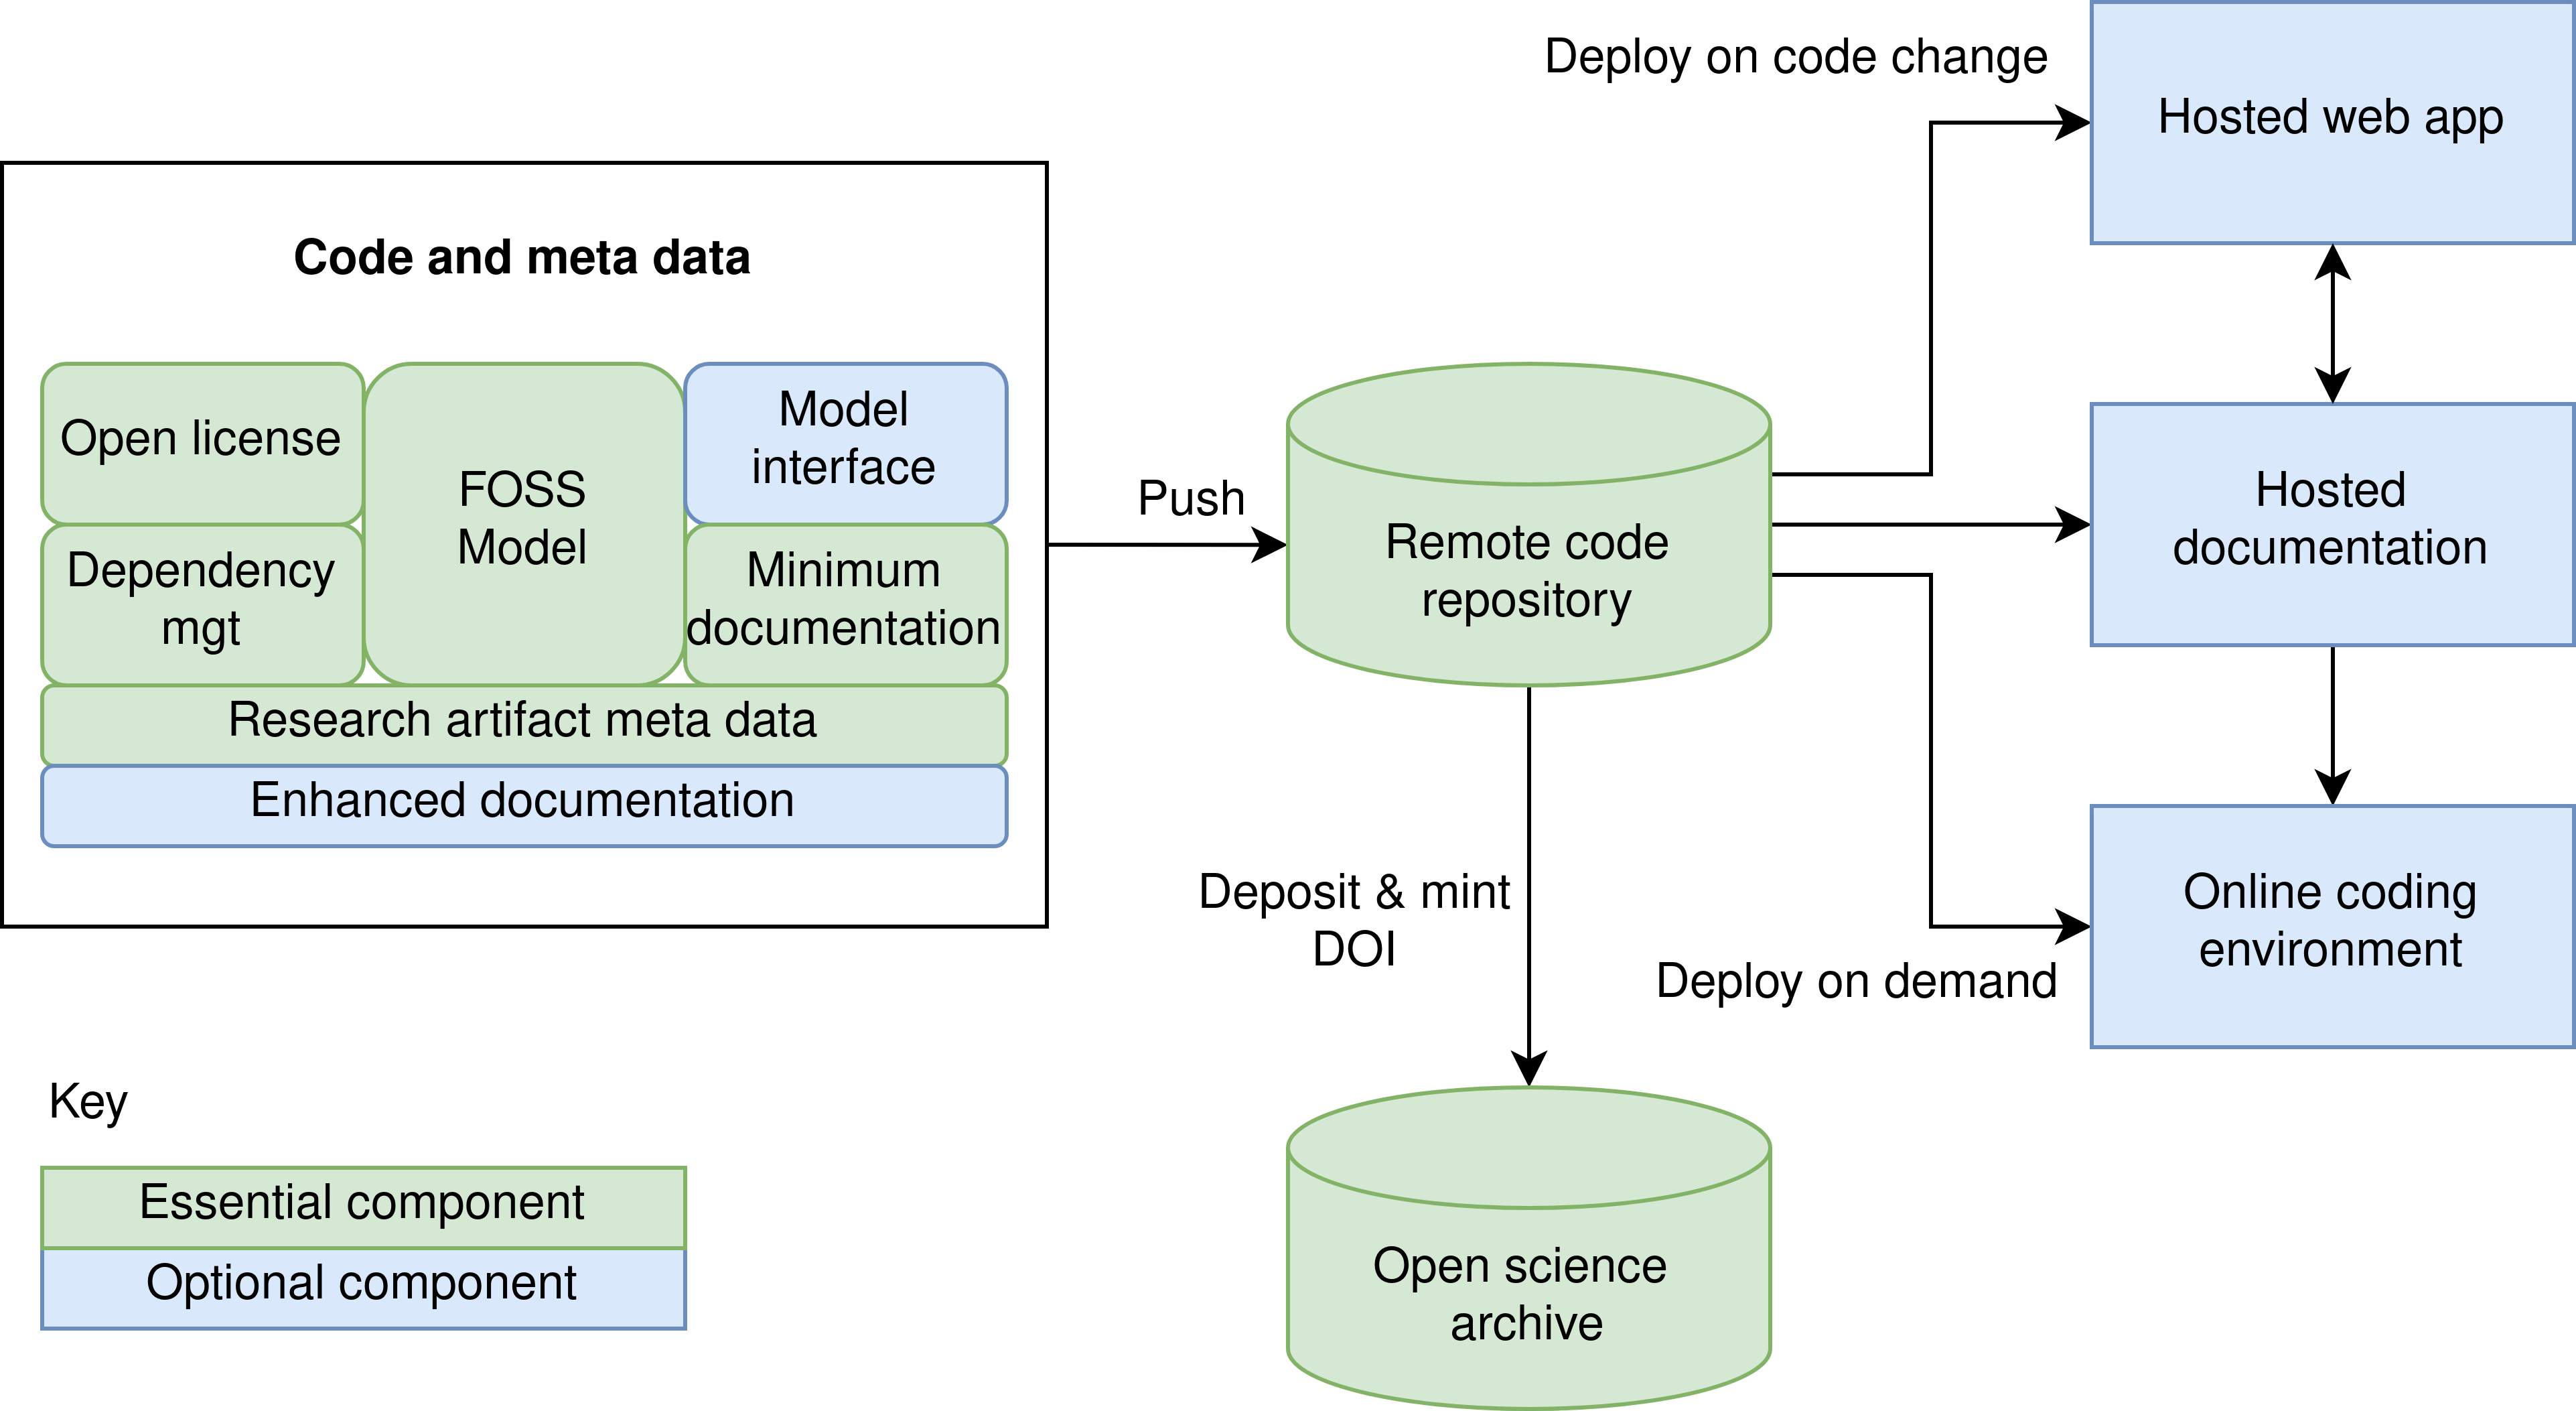
\includegraphics[scale=0.85]{images/stars_framework_overview.png}
    \caption{An overview of the STARS framework. Components shaded blue are optional: used depending on project requirements, skills, time available, and experience of team.}
    \label{fig:overview}
\end{figure}

\section{Description of Framework Components}

We recognise that open science takes additional work. Therefore we designed the STARS framework (Figure \ref{fig:overview}) to divide work into \textit{essential} and \textit{optional} components. The essential components provide the minimum work needed to share DES models to allow them to be available long-term, citable, functional, appropriately licensed, and likely to be at a standard that is reusable in further work  (shaded green in Figure \ref{fig:overview}).  The \textit{optional} components of the STARS framework focus on enhancing the accessibility, understanding, and maintainability of FOSS simulation models  (shaded blue in Figure \ref{fig:overview}).  In this section, we provide a general description of the components.  The following section includes three applied examples and to support understanding we translate Figure \ref{fig:overview} into a simple list of components (see Table \ref{tab:applied_examples}).

\subsection{Essential components}

 We designed the \textit{essential} components to support authors to meet the requirements of two ACM badges if tested in an RCR: `artefact available'; and `artefacts evaluated - functional'. A study implementing the essential components would meet the majority of the best practices evaluated by \cite{monks2023computer}.

\subsubsection{Open license}
Before sharing (or making any code public), it is necessary for authors to select an appropriate FOSS license for the code and other research artefacts.  This ensures appropriate use of the model, and if needed removes legal liability of the authors. A common approach in data science and other computational fields is to adopt a permissive license such as the MIT, but other options exist.  For example, a model could be made available under a GNU Public Licence (GPL). The GPL is an example of a copyleft license: where the rights granted must be preserved in all derivative works (typically by publishing under the same GPL license).  Without a license, the model is available, but not (re)usable.  Authors retain exclusive copyright and any derivative works are at risk of a take down request from the original authors.

Adding a license to a simulation project is a minor task. For support selecting a license and for license text we recommend consulting the online resources provided by `Choose an Open Source License'\footnote{\url{https://choosealicense.com/}}. Popular online code repositories such as GitHub and GitLab also provide templates and simple workflows to automatically add licenses to a project.


\subsubsection{Dependency management}
For any type of software or code deployment problem it is necessary to adopt a language that allows model developers to specify the software libraries, version numbers and sources that are required in order for the model to run. Without this information the likelihood of others being successful in reusing models is greatly reduced as models will generate missing dependency error that researchers will be required to solve.  \cite{monks2023computer} found that the vast majority of healthcare authors that coded their DES models did not make use of formal dependency management.   

If we take a popular FOSS language such as Python for example, three well known options for managing dependencies exist: pip virtual environments, conda environments, and poetry. Each of these approaches allow a user to accurately record the key Python software used in the project. In turn the dependency management tools then reconcile the dependencies required for this software. For example, conda virtual environment document dependencies in the \textit{Yet Another Mark-up Language (.yml)} format. 

Once learnt, using a dependency management tool is a simple task and has low time overhead to setup. Our experience is that dependencies may change during a project and that some rework of environment files is needed during the project (as dependencies are added or removed) along with a final check at the end.

\subsubsection{DES model}
The STARS framework is designed to be general to any DES model coded in a FOSS simulation package; for example, using R, Julia or Python. In our application exemplars, we demonstrate different ways to use the framework using two popular simulation packages in Python: \textit{Simpy} and \textit{Ciw}. There are no formal requirements within STARS for how a model is structured or implemented.  We do recommend that modellers aim to keep model code independent of any \textit{front-end} and is executable standalone. Guidance and support for how setup could be achieved in Python is available elsewhere \citep{monks2023improving, tom_monks_2023_8101984}. 

\subsubsection{Minimum documentation}

Within the STARS framework, DES models are shared with a set of minimal instructions that provide an overview of what a model does, how to install and run the model to obtain results, and how to vary parameters to run new experiments. A simple way to achieve this is a README file.  In data science projects, this information is often contained in a markdown file in the root directory for the modelling project (i.e. README.md). An advantage of this approach is that online code repositories (GitHub/GitLab/BitBucket) show the contents of this file as part of the project's webpage, that is, users do not need to download the documentation, they can read it online.

\subsubsection{Research artefact meta-data}

A model shared using STARS is stored with data describing the researchers and the artefact. STARS requires two basic items of meta-data. The first are the Open Researcher and Contributor IDs (ORCID) for each study author. An ORCID is a unique identifier for a researcher; it provides a permanent link back to an authors publication (including related publications) and funding history. For example, the lead author of this papers ORCID is 0000-0003-2631-4481 and their details can be accessed via https://orcid.org/0000-0003-2631-4481. A minimal implementation to store this information is to include researcher ORCIDs in the README.md file.

While it is easy for a researcher to cite an academic paper, it may appear less obvious how to cite a model archive (e.g. model code). The second requirement is therefore citation information for the research artefact i.e. a way to provide credit to the author, and direct readers to original code, if the work or derivatives are used in any future study. A solution is to create CITATION.cff file that contains all the citation information for the model and code artefacts (e.g. name, authors, version).  This approach is support by remote code repositories (e.g GitHub), Open Science Archives (we shall describe these shortly) and some reference management software tools.  There are online tools to support the creation of CITATION.cff files \citep{druskat_stephan_2021_5171937}. The next section provides three applied examples implementing CITATION.cff and links to authors via ORCIDs.

\subsubsection{Remote code repository}
Central to Figure \ref{fig:overview} is a remote code repository. The most popular solutions are GitHub\footnote{\url{https://docs.github.com/en}}, GitLab\footnote{\url{https://about.gitlab.com/}}, and BitBucket\footnote{\url{https://bitbucket.org/}}. GitHub and other online code repository’s primary purpose is version control of code.  That is, modellers incrementally commit updates to their code and models during development. These tools allow for easy \textit{rollback}, inspection, or use of older versions of the code. Another major feature of version control is \textit{branching}. The main (sometimes called master) branch of a repository contains the production model i.e., a simple, but functional simulation model that can be deployed to users.  Incremental developments are typically made on a development or feature branch, tested and then merged into the main branch when a modeller is confident it will not break the production model. GitHub is an online tool.  In traditional workflows, all of the model coding is done offline in a local code repository that is managed by a local version control system such as Git. A modeller codes their model on their own machine, and \textit{pushes} their commits to GitHub (or a similar repository). A new user of the code would \textit{clone} the GitHub repository to their own local machine. A user who is already using the code might \textit{pull} updates from the remote repository and \textit{merge} changes into their own branch.

As a simple example, consider a model of an emergency department (ED) developed in the Python DES package SimPy. The model logic is fully coded and it can be run from the command line. The working SimPy model is currently committed to the main branch. A researcher can \textit{clone} the main branch of the repository and execute the model to analyse the ED in their study. Simultaneously, a simulation modeller can develop a graphical interface for the model on a separate feature branch (e.g. called \textit{interface}). When the interface is complete the modeller can issue a pull request to the main branch.  A pull request is effectively a request to merge code from one branch into another e.g. from \textit{interface} to main.  It provides a safety net for the changes to be reviewed before merging (and potentially breaking a production model). Once merged the researcher can simply pull the new code from the main branch, although there are no guarantees the new model interface will install easily on the researcher's machine.

A secondary use of online code repositories is for collaboration on scientific studies and model development. These solutions provide many mechanisms for its users to share, review, and control code. One simple example is \textit{Issues}. This is a discussion log that might report bugs, potential improvement, new ideas, and general queries. Another example is the concept of a \textit{release}. A release tags a snapshot of the code. In our ED model example, the SimPy command line model might be tagged as version 1.0.0. While the ED model with a graphical user interface might be tagged as version 2.0.0. A release is an easy way for modellers to talk to their users about the correct version of the model: it supports a shared language between modellers and users.

\subsubsection{Open Science archive}

 Our last essential component is for long-term archiving (and preservation) of simulation models. Our framework links code in the remote repository to an open science archive that has FORCE11 compliant citation \citep{smith_software_2016} and guarantees on persistence of digital artefacts by adhering to TRUST principles \citep{lin_trust_2020}. Examples, include Figshare\footnote{(\url{https://figshare.com/})}, Zenodo\footnote{(\url{https://zenodo.org/})}, the Open Science Framework\footnote{(\url{https://osf.io/})}, and the Computational Modeling in the Social and Ecological Sciences Network (CoMSES Net)\footnote{\url{https://www.comses.net/})}. Each of these archives has guarantees on storage and mints Digital Object Identifiers (DOIs) to enable citation and, includes meta-data to improve discoverability.  In the long term, open science archives hold significant advantages over remote code repositories. For example, code in a GitHub repository could change over time, be made private, or be deleted.
 
 As an example consider the orthopaedic planning simulation model code published by \cite{alison_harper_2023_8011462}. The model has been deposited in Zenodo and has been allocated the DOI \textit{10.5281/zenodo.7900852} (accessed via \url{https://zenodo.org/record/8011462}).  This artefact is citable in the same way as a journal article and uses ORCID meta-data to link the work to the authors research portfolio. 

Depositing models in open science archives fits seamlessly into the journal article publication lifecycle using versioning. Before a manuscript is submitted to a journal, the model code is deposited, a DOI is minted, and the artefact is cited in the article.  If changes are required to the model code after the initial peer review these are then re-deposited, a new DOI is minted for the artefact, and the new deposit is cited in the revised article.  The deposit is automatically linked back to the previous version using the original DOI. 


\subsection{Optional components}

The \textit{optional} components of the STARS framework focus on enhancing the accessibility, understanding, and maintainability of FOSS simulation models  (shaded blue in Figure \ref{fig:overview}).  Users may include one or more of the optional components to improve the likelihood of their simulation model being reused. We designed the optional components to support healthcare simulation authors to meet the requirements of one ACM RCR badge: `artefacts evaluated - reusable'.

\subsubsection{Enhanced documentation}
\label{enhanced_docs}

The STARS framework advocates that any simulation used for health decision making should provide open and high quality documentation on how the model is implemented and works. We encourage users to adopt contemporary FOSS tools to support the creation of these materials.  

A simple solution is to adopt Jupyter notebooks for documenting a model.  Project Jupyter is a FOSS project that supports scientific coding in Python, \textit{R} and Julia in a classical notebook format.  A simple way to conceptualise Jupyter notebooks are as a browser based interface and an execution kernel.  The interface provides a set of markdown and code cells that a user can control. Markdown is simply a way to present formatted text, mathematics, and code together. Notebooks provide a way to explain, document and execute simulation experiments. For example, an analyst may have created a set of Jupyter notebooks for model validation, determining the number of replications, warm-up analysis, defined experiments, or interactive experimentation.  

Jupyter's kernel executes all of the code.  Typically the kernel is located on the users local machine, but given the server nature of Jupyter, the kernel could be located on a remote (possibly powerful) machine.  In these remote cases the user need not have the FOSS simulation package or Jupyter installed on their own machine.


Notebook and markdown files containing simulation model code and documentation can be brought together using contemporary publishing software. Two examples are Quarto \footnote{(\url{https://quarto.org/})} and Jupyter Book \footnote{(\url{https://jupyterbook.org})}.  These are high level tools that offer different ways to collate and publish documentation. For example, both can be used to create a structured website. This provides researchers the opportunity to construct a detailed book that could be hosted online for their simulation study with the aim of supporting simulation model understanding and appropriate reuse. While the STARS framework is not prescriptive about the content included in enhanced documentation, authors are encouraged to consider some or all of the following areas:

\begin{itemize}
    \item A plain English summary of the project context, and model;
    \item Clarifying simulation model open licensing terms;
    \item Clear citation instructions for the model and documentation;
    \item Instructions for how others can contribute (e.g. code, bug fixes, modifications, improved documentation), and report issues to the project;
    \item Instructions for installing and using the model;
    \item A structured code walk through of the model;
    \item Documenting the modelling cycle using TRACE \citep{TRACE_2021}; 
    \item Annotated simulation reporting guidelines e.g. the STRESS-DES.
    \item A clear description of model validation including its intended purpose.
\end{itemize}

% In our example, we provide a link to another web based technology: a Jupyter Book deployed in GitHub pages \url{https://tommonks.github.io/treatment-centre-sim}.  

\subsubsection{Documentation hosting}

STARS users could, as an option, choose to host their enhanced documentation online using a free web hosting service. At the time of writing, there are multiple secure stable services  for serving static content; for example, GitHub Pages (owned by Microsoft)\footnote{\url{https://support.atlassian.com/bitbucket-cloud/docs/get-started-with-bitbucket-cloud/}}, GitLab Pages\footnote{\url{https://docs.gitlab.com/ee/user/project/pages/}}, BitBucket Cloud\footnote{\url{https://support.atlassian.com/bitbucket-cloud/docs/get-started-with-bitbucket-cloud/}}, or Quarto Pub (for Quarto created content)\footnote{\url{https://quartopub.com/}}. Although all of these services have limits on their usage, they would be suitable for a healthcare simulation project; for example, at the time of writing GitHub pages has a limit of 1GB of content and a \textit{soft} bandwidth of 100GB per month. In our applied examples the largest website hosting enhanced documentation was $<$ 5MB in size. This would allow for more than 20,000 visits per month, assuming all site pages were visited by each user, before soft limits were reached.  

These services offer a way to publish companion enhanced documentation with a research article. However, STARS recognises the transient nature of technology and all enhanced documentation should be deposited in an Open Science archive to guarantee its longevity and maintain a snapshot of the documentation at the time of article publication.   

\subsubsection{Online coding environment}

Jupyter's use of the browser and ability to run code on a remote kernel allows for easy deployment of simulation notebooks to a technical user-base. In the UK for example, these may be well trained NHS analysts from the NHS-Python / NHS-R community or other researchers familiar with reading and running code.  In summary, an optional component of the STARS framework is to provide an online environment where users can run and change code. 

A FOSS solution for deployment is to make use of a BinderHub such as \url{mybinder.org}. A BinderHub provides a Jupyter environment in the cloud that others can use to run your simulation model.  One simple requirement is that the FOSS simulation model code, and Jupyter notebooks are available in a public code repository hosted in the cloud; e.g. on GitHub or GitLab. Binder works by on-demand containerisation of a code repository and code and deployment. In computing, containers refer to lightweight, portable, self-contained software units that package together an application, such as a simulation model, and all its software dependencies, including libraries, frameworks, data, and system tools. Within STARS, for example, this would make use of the essential dependency management approached used (e.g. conda) to install the necessary libraries to run the model on a linux operating system and then deploy to the binder web server. 

One advantage of a BinderHub approach is that it can integrate with enhanced documentation components of STARS.  For example, a notebook that is part of a Jupyter Book can become interactive at the click of a button. 

In addition, to Binder's FOSS solution, proprietary online notebook alternatives also exist. For example, Google Colaboratory\footnote{\url{https://colab.google/}} or Deepnote\footnote{\url{https://deepnote.com/}}.  These are closed source, but offer both free and paid tiers of service.  Unlike BinderHub the software environment is not specified before launch.  For example, a user would need to attempt to install a simulation package after a notebook has been opened.


\subsubsection{Model interface}

A web application (web app) interface to the model is accessible to less technical simulation users such as healthcare analysts, healthcare managers, researchers not familiar with Python or R, or the general public. A web app will provide simple ways to setup and execute the model. This might include parameter fields, logic diagrams, basic animation, and buttons.   

For example, in Python there are multiple solutions available to create an interface for a model e.g. Streamlit \citep{streamlit}, Shiny for Python \citep{shinypy}, or plotly dash \citep{shammamah_hossain-proc-scipy-2019}. An important point to note here is that there is no requirement that model interfaces are hosted on a web server. They are browser based technology and, just as enhanced documentation, can equally be installed and run on a laptop or desktop. This opens STARS up to different types of project including supporting private code - for ethical or governance reasons - but shared between a project team.  

Each solution provides its own API for screen widgets (e.g. sliders, results tables, buttons) as well as unique benefits and downsides for simulation.  
If deployed to a web app hosting service then the simulation models become much more accessible; for instance they are designed to display and be usable via phones, and other mobile devices. This brings us to the final optional component for deploying web apps online.  

\subsubsection{Web app hosting}

In healthcare simulation, online deployment of computer models, opens a new channel for the FOSS community to work with busy clinicians and health professionals.  For example, a simulation researcher working with a paediatric consultant, could prototype a web app containing a simulation model of a children's emergency department, using Python and streamlit; deploy to an online host, and message the consultant the URL. The busy consultant can then review when they are free, perhaps on their phone, and message back with feedback.

Web app software, such as streamlit, or Shiny, may have its own free tier of hosting.  For example, StreamLit community cloud is a free hosting service for Streamlit apps. When used together they provide a robust and easy way to share simulation models to healthcare users. As it is the aim of these services, deployment of apps is often trivial. For example, Streamlit Community Cloud only needs to be given access to a GitHub repository and it copies the code, builds the app and deploys to a user customised URL. As with BinderHub, the free tier of any web app hosting service has limitations; typically in the number of processors available, memory and/or monthly bandwith.  If required, services like ShinyApps offer monthly paid plans to increase computational resources.  If apps are not used for an extended period then service providers often suspend the app.  The next user that accesses the URL then faces a short wait while the app wakes up.

\section{Applied examples in Python}

To demonstrate the feasibility of our framework and support researchers in its use, we provide three applied examples. In each example we vary the technology, approach, and degree of effort (implemented components), to illustrate the flexibility available to researchers. For example, varying the open license, Python simulation software, web application, documentation tools and hosting.  Table \ref{tab:applied_examples} lists all components from Figure \ref{fig:overview} and summarises the tools used in each example to share research artefacts against essential and optional enhanced framework components.  For simplicity we also summarised the artefacts archived in Zenodo in Table \ref{tab:artifacts}




% table 2
\begin{table}[htp!]
\tbl{Implementation of the framework across three examples}
{\begin{tabular}{lllll} \toprule
\multicolumn{2}{l}{\textbf{STARS Components}}                                    & \textbf{Applied example 1} & \textbf{Applied example 2} & \textbf{Applied example 3} \\ 
\hline \\
\multirow{7}{*}{\textit{\textbf{Essential}}}     & \textit{1. Open License}              & MIT                                                          & MIT                                                          & GNU Public License 3                                         \\
                                            & \textit{2. Dependency mgt}            & conda                                                       & conda                                                        & conda                                                        \\
                                            & \textit{3. DES software}              & simpy                                                        & simpy                                                        & ciw                                                          \\
                                            & \textit{4. Code repository}           & GitHub                                                       & GitHub                                                       & GitHub                                                       \\
                                            & \textit{5. Meta-data}                 & citation.cff + ORCID & 
                                            citation.cff + ORCID & citation.cff + ORCID \\
                                            & \textit{6. Minimum documentation}     & README.md                                                    & README.md                                                    & README.md                                                    \\
                                            & \textit{7. Open science repository}   & Zenodo                                                       & Zenodo                                                       & Zenodo                                                       \\ \hline \\
\multirow{5}{*}{\textit{\textbf{Optional}}} & \textit{8. Online coding environment} & Binder                                                       & Binder                                                       & Binder                                                       \\
                                            & \textit{9. Enhanced documentation}    & Electronic Notebook                                          & Jupyter Book + STRESS                                                & Quarto + STRESS                                                      \\
                                            & \textit{10. Documentation hosting}    &                                                              & GitHub pages                                                 & GitHub pages                                                 \\
                                            & \textit{11. Model interface}          &                                                              & streamlit                                                    & Shiny for python                                             \\
                                            & \textit{12. Web app hosting}          &                                                              & streamlit community cloud                                    & shinyapps.io \\   
                                            \bottomrule
\end{tabular}}
\label{tab:applied_examples}
\end{table}





% Please add the following required packages to your document preamble:
% \usepackage{multirow}
% table 3
\begin{table}[htp!]
\tbl{Simulation artefacts and archives from the applied examples}
{\begin{tabular}{ll}
\toprule
\textbf{Example 1}                 & \textbf{URL}                                                                               \\ \hline
Code repositories                  & \url{https://github.com/pythonhealthdatascience/stars-treat-sim}          \\ 
Archive and DOIs & \url{https://doi.org/10.5281/zenodo.10026327} \\
                                   & \\ \hline
\textbf{Example 2}                 & \textbf{URL}   \\ \hline
\multirow{2}{*}{Code repositories} & \url{https://github.com/pythonhealthdatascience/stars-streamlit-example}  \\  
                                   & \url{https://github.com/pythonhealthdatascience/stars-simpy-example-docs} \\ 
Web app                            & \url{https://stars-simpy-example.streamlit.app}                           \\ 
Documentation                      & \url{https://pythonhealthdatascience.github.io/stars-simpy-example-docs}  \\ 
                                  
\multirow{2}{*}{Archive and DOIs} & \url{https://doi.org/10.5281/zenodo.10055169}  \\  
                                   & \url{https://doi.org/10.5281/zenodo.10054063} \\ 
                                   & \\ \hline
\textbf{Example 3}                 & \textbf{URL}                                                                               \\ \hline
Code repositories                  & \url{https://github.com/pythonhealthdatascience/stars-ciw-example}        \\ 
web app                            & \url{https://pythonhealthdatascience.shinyapps.io/stars-ciw-examplar}     \\ 
Documentation                      & \url{https://pythonhealthdatascience.github.io/stars-ciw-example}         \\

Archive and DOIs & \url{https://doi.org/10.5281/zenodo.10051495}
\\ \hline
\end{tabular}}
\tabnote{All artefacts are archived in Zenodo.  Follow links to find version of code at time of submission to the Journal of Simulation.}
\label{tab:artifacts}
\end{table}






\subsection{Python DES packages}

The advantages of Python for simulation modelling, including its simplicity and readability, have been described in \cite{dagkakis2016review}. The Python data science ecosystem contains a large number of modules, libraries and frameworks for supporting analysis, flexible modelling, and integration of simulation with other methods such as optimisation, machine learning, and visualisations. 

In our applied examples, we employ two Python DES FOSS packages: \textit{Simpy} \citep{simpy} and \textit{Ciw} \citep{ciw}.  We chose these packages as they are both maintained, have recent publications using or developing them, and adopt permissive open licensing.

\textit{Ciw} was developed with a focus on reproducibility, and best practice in terms of documentation, readability, transparency, version control, and testing. It allows users to very quickly build complex multi-class queuing networks. It is modular and modifiable, and by integrating with the Python ecosystem, several examples of open hybrid simulations have been implemented \citep{palmer2023implementing, palmer_geraint_2021_4601529}. \textit{Ciw} has been used for applied healthcare simulation modelling, for example for planning large-scale outpatient services \citep{zou2022impact}. 

\textit{Simpy} is the most commonly used Python DES package. It is easily mixed with standard Python and runs using Python generator syntax.  \textit{Simpy} has been used in several open-source OR-relevant publications \citep{allen_simulation_2020, Chalke043795, harper2023post, lim2020staff, cubukcuoglu2020discrete}.


% There are several well-maintained Python packages available for building FOSS DES models, which vary in terms of features, complexity, and focus.

% In their review of open source software for DES, \cite{dagkakis2016review} identified three FOSS Python packages: \textit{Simpy} \citep{simpy}, \textit{Pysimulator} \citep{pfeiffer2012pysimulator} and \textit{ScipySim} \citep{mcinnes2011scipysim}. The authors subsequently developed their own software library for DES with a focus on manufacturing environments, \textit{ManPy} \citep{dagkakis2016manpy}, built using \textit{SimPy}. \textit{ManPy} is not currently maintained. \textit{PySimulator}, and \textit{ScipySim} were last updated in 2014, and 2010 respectively, while \textit{SimPy} has continued to be maintained, with a new release in June 2023. An updated list of Python DES packages now includes \textit{Salabim} \cite[MIT licensed, last updated July 2023]{van2018salabim} and \textit{Ciw} \cite[MIT licensed; last updated April 2023]{ciw}.


% MOVE THIS SECTION TO DISCUSSION
% \textit{Salabim} contains many simulation tools including automatic results collection and animation. Using \textit{Salabim}, \cite{shoaib2022simulation} developed an open-source, generic model of a primary care network. The simulation is reconfigurable, and the authors demonstrate its widespread applicability for model reuse. with a focus on manufacturing environments, \textit{ManPy} \citep{dagkakis2016manpy} was built using \textit{SimPy}. 


\subsection{Applied example 1: a minimal implementation}

Our first example is a minimal implementation of the STARS framework. We use all essential components to enhance a \textit{Simpy} simulation model. We then further enhance the model by creating a Jupyter notebook containing an annotated explanation of each section of code in the model and instructions to run the model. We made the notebook executable online using Binder.  

\subsubsection{Case study model}

We adapt a textbook example from \citet[p.170]{nelson2013}: a terminating DES model of a U.S based treatment centre. In the model, patients arrive to the health centre between 6am and {\color{red}midnight} following a non-stationary Poisson process. On arrival, all patients sign-in and are triaged into two classes: trauma and non-trauma. Trauma patients include impact injuries, broken bones, strains or cuts etc. Non-trauma include acute sickness, pain, and general feelings of being unwell etc. Trauma patients must first be stabilised in a trauma room. These patients then undergo treatment in a cubicle before being discharged. Non-trauma patients go through registration and examination activities. A proportion of non-trauma patients require treatment in a cubicle before being discharged. The model predicts waiting time and resource utilisation statistics for the treatment centre. The model allows managers to ask question about the physical design and layout of the treatment centre, the order in which patients are seen, the diagnostic equipment needed by patients, and the speed of treatments. For example: “what if we converted a doctors examination room into a room where nurses assess the urgency of the patients needs.”; or “what if the number of patients we treat in the afternoon doubled”

\subsubsection{Software environment}

We used Python 3.8. Data manipulation, simulation, and general mathematical modeling were done using Simpy v4.0.1 \citep{simpy}, NumPy v1.19.2 \citep{numpy} and Pandas v1.2.3 \citep{mckinney2011pandas}. Charts were produced with MatPlotLib v3.3.4 \citep{Hunter:2007}. Enhanced documentation was created using Jupyter-Lab v2.4.3 \citep{jupyterlab_jupyterlab_2022}.

\subsubsection{Implementation of essential framework components}

We used a GitHub repository to host and version control our production code (\url{https://github.com/pythonhealthdatascience/stars-treat-sim}). All core computational materials  (Figure \ref{fig:overview})  have been made available under an MIT permissive license.  Any users of the research artefacts and DES model are free to re-share the model under any terms they choose including commercial, but they must cite the authors and accept that the authors do not have any liabilities. We made the Python software environment explicit and reproducible using the conda package manager. Basic documentation is provided using a a README file i.e. basic instructions for installing and running the model are contained in the README file that is seen when navigating to the GitHub repository URL.  Our README file also contains markdown badges displaying the authors ORCIDs and are hyperlinked to the authors' individual ORCID records. We then archived all essential components for this publication (all contained with the GitHub repo) in Zenodo. The materials are citable using DOI: \textit{10.5281/zenodo.10026327} \citep{applied_example1}.

\subsubsection{Optional components: documentation and online interactive code}

In our minimal example, we first enhanced model documentation using a Jupyter Notebook.  The notebook breaks down the code for model inputs, logic and usage into sections and provides a detailed explanation of each.  

Given that we had created a notebook, we used Binder to provide an online instance of Jupyter Lab for expert users to run the model's Python code without the need to install any software on their local machine.  Binder expects that a conda virtual \verb|environment.yml| file is placed into a sub-directory \verb|binder/|. Once this has been committed it is a simple case of navigating to \url{https://mybinder.org/} and copy and pasting the URL into the build and launch text box. Binder will then create a remote instance that contains both the code and dependencies specified in the \verb|binder/environment.yml| file.  The first time the instance is built it will likely take several minutes.  This process may  need to be repeated if the instance is not used regularly or code is changed.

A model instance can be launched on Binder from the Github repository. A user need only click on the badge in the README file labelled "Launch Binder". The model notebook can be found \verb|src/full_model.ipynb|.  You will be presented with a notebook; an example is in Figure \ref{fig:jupyter}.

\begin{figure}[ht]
\centering
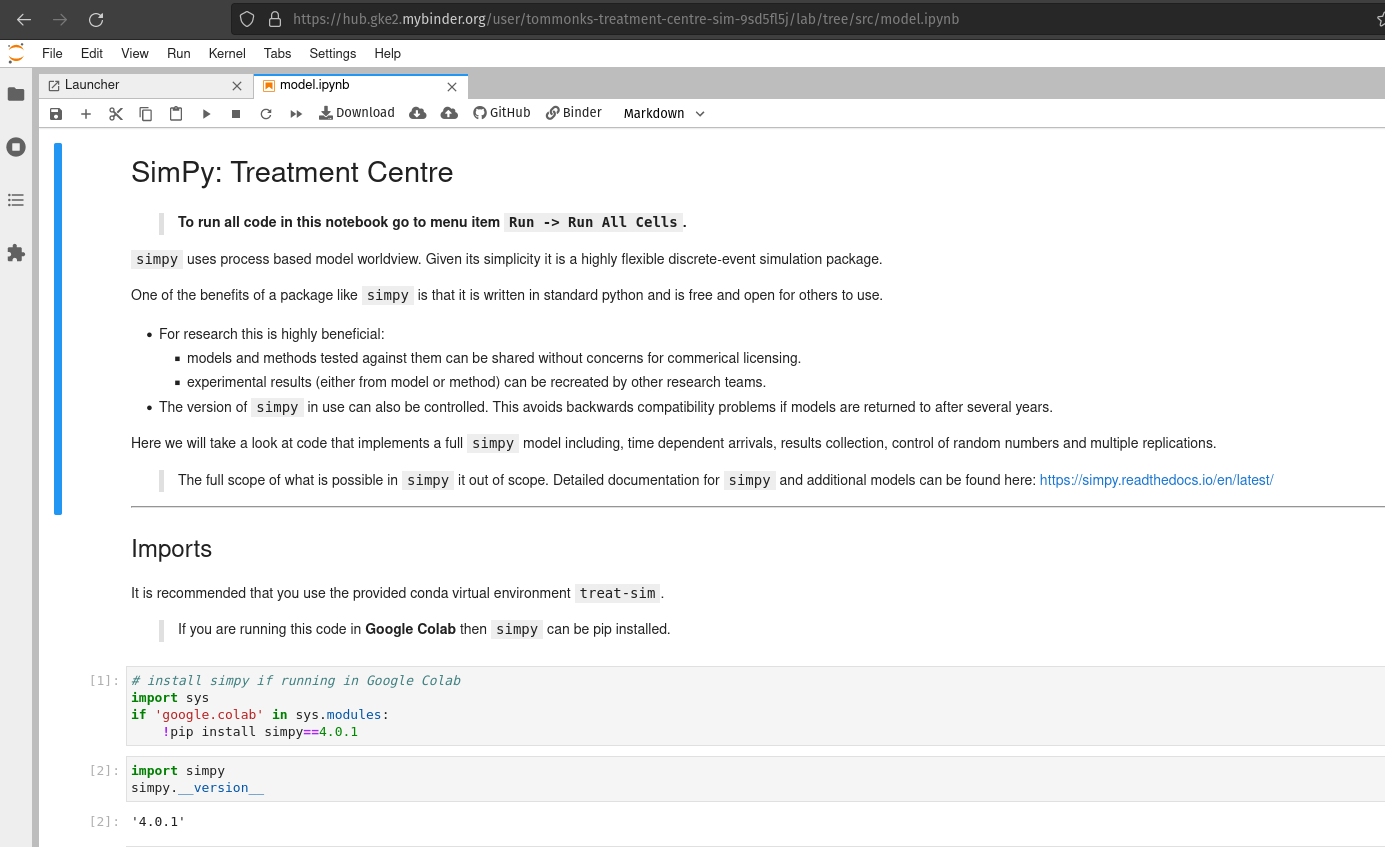
\includegraphics[scale=0.25]{images/jupyter.png}
\caption{Simulation model and Jupyter lab running in Binder}
\label{fig:jupyter}
\end{figure}

\subsection{Applied example 2}

Applied example 2 is again based on essential STARS framework components from example 1 (using the treatment centre case study model) and fully implements the optional components including enhanced documentation that is hosted online, and a web app to support usability (Figure \ref{fig:overview}).  We created a new GitHub repository to host our essential components and model interface (\url{https://github.com/pythonhealthdatascience/stars-streamlit-example}).

% \subsubsection{Case study model}

% We adapt a textbook example from \citet[p.170]{nelson2013}: a terminating discrete-event simulation model of a U.S based treatment centre. In the model, patients arrive to the health centre between 6am and 12am following a non-stationary Poisson process. On arrival, all patients sign-in and are triaged into two classes: trauma and non-trauma. Trauma patients include impact injuries, broken bones, strains or cuts etc. Non-trauma include acute sickness, pain, and general feelings of being unwell etc. Trauma patients must first be stabilised in a trauma room. These patients then undergo treatment in a cubicle before being discharged. Non-trauma patients go through registration and examination activities. A proportion of non-trauma patients require treatment in a cubicle before being discharged. The model predicts waiting time and resource utilisation statistics for the treatment centre. The model allows managers to ask question about the physical design and layout of the treatment centre, the order in which patients are seen, the diagnostic equipment needed by patients, and the speed of treatments. For example: “what if we converted a doctors examination room into a room where nurses assess the urgency of the patients needs.”; or “what if the number of patients we treat in the afternoon doubled”

% \subsubsection{Software environment}

% We used Python 3.8. Data manipulation, simulation, and general mathematical modeling were done using Simpy v4.0.1 \citep{simpy}, NumPy v1.19.2 \citep{numpy} and Pandas v1.2.3 \citep{mckinney2011pandas}. Charts were produced with MatPlotLib v3.3.4 \citep{Hunter:2007}. All analyses were conducted in Jupyter-Lab v2.4.3 \citep{jupyterlab_jupyterlab_2022}. The web app was produced using streamLit v1.13.0 \citep{streamlit}.  Enhanced documentation was created using Jupyter Book v0.13.1 \citep{executable_books_community_2020_4539666}. 

% \subsubsection{Implementation of essential framework components} [SHRINK ]

% % should I rename the repository to STARS-applied-examplar2 ????
% . All core computational materials have been made available under an MIT permissive license.  Any users of the research artefacts and DES model are free to re-share the model under any terms they choose including commercial, but they must cite the authors and accept that the authors do not have any liabilities. We made the python software environment explicit and reproducible using the conda package manager. Basic documentation is provided using a combination of a README file and a Jupyter notebook; i.e. basic instructions for installing and running the model are contained in the README file that is seen when navigating to the GitHub repository URL.  Our README file also contains markdown badges displaying the authors that display the authors ORCIDs and are hyperlinks to the authors individual ORCID records.  All core components for this publication are archived in Zenodo and citable using DOI: \textbf{todo} (\textbf{cite}).

\subsubsection{Web app: Streamlit}

Our web app is implemented in \textit{streamlit} and hosted on streamlit's free community cloud (\url{https://stars-simpy-example.streamlit.app}).  We have provided a multi-page application allowing users to switch between an interactive simulation, a fixed set of reproducible experiments, custom batches of experiments, and an ``about" page providing information and links to enhanced documentation. Deployment of the web app is controlled by linking a streamlit community cloud account to our GitHub repository.  Figure \ref{fig:app} illustrates the interactive page from the web app: users can manipulate model parameters using sliders and are presented with results.

Live code for the streamlit interface to the model is available under the MIT license in GitHub. Code is also archived in Zenodo and citable using DOI \textit{10.5281/zenodo.10055169} \citep{applied_example2_app}




% I might include a new image. This will do for now.
\begin{figure}[ht]
\centering
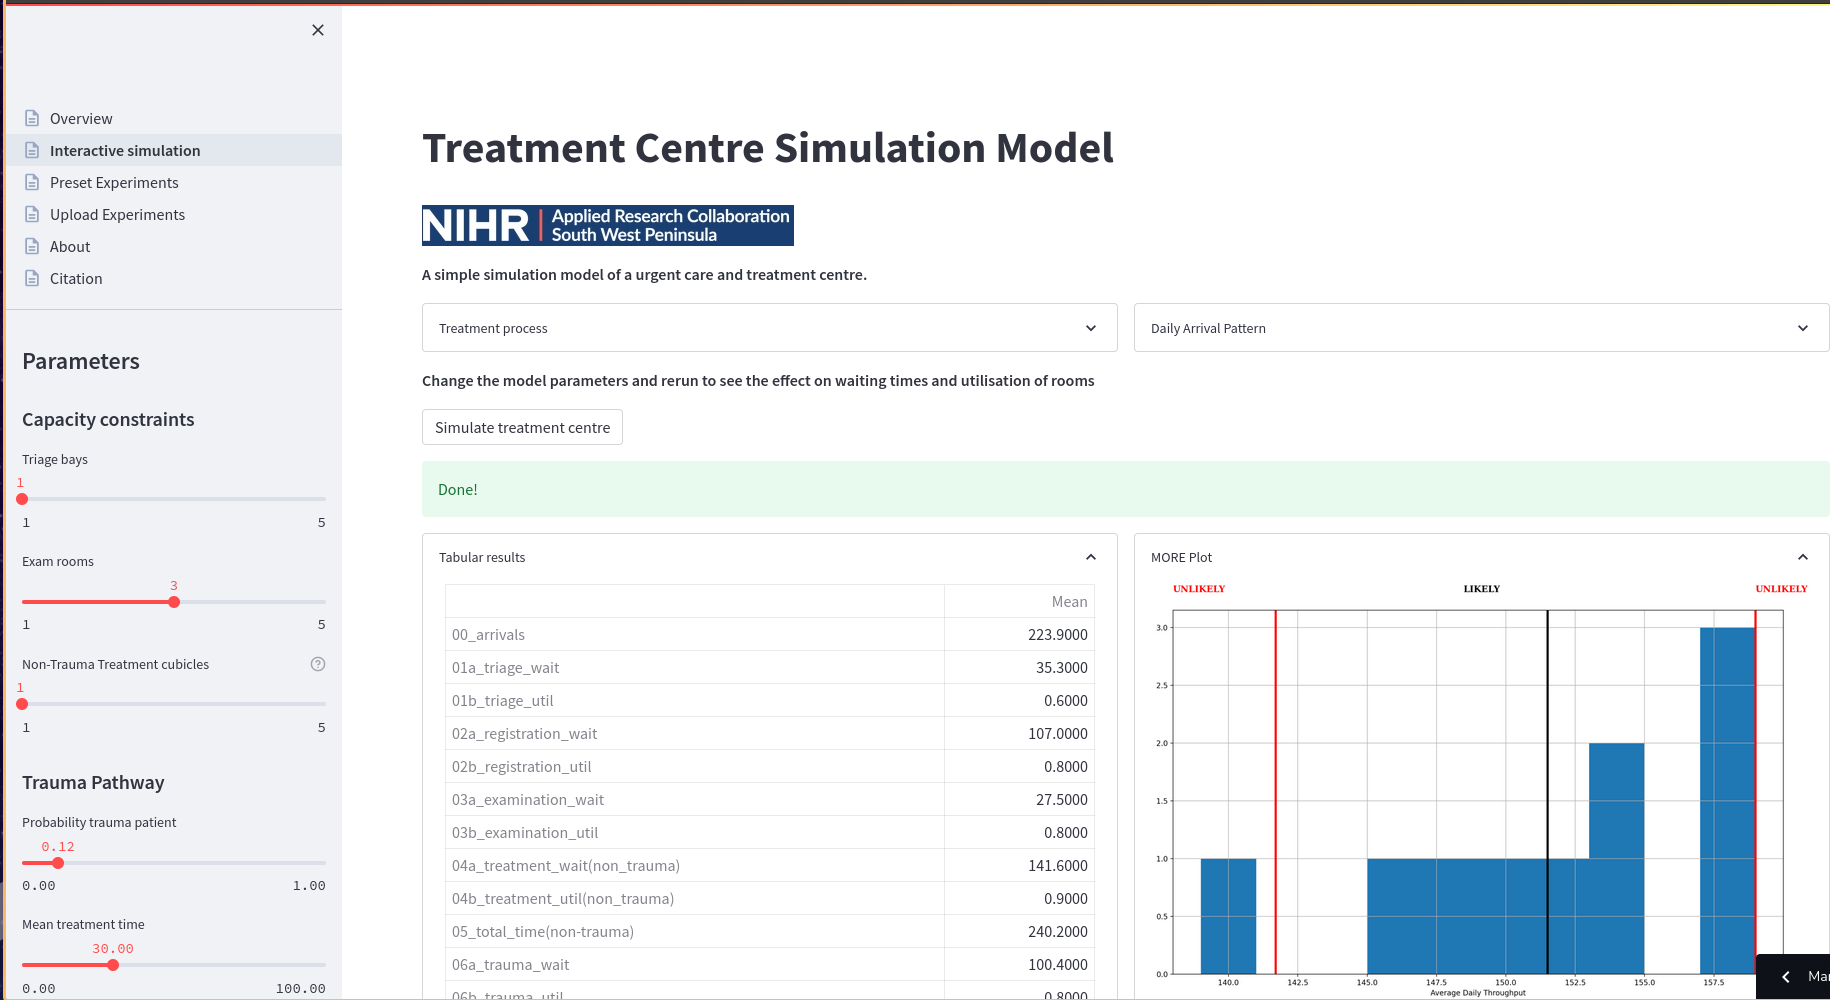
\includegraphics[scale=0.18]{images/web_app_screenshot.png}
\caption{Treatment centre user interactive simulation  }
\label{fig:app}
\end{figure}


\subsubsection{Enhanced documentation: Jupyter Book}

For our documentation we created a second Github repository \url{https://github.com/pythonhealthdatascience/stars-simpy-example-docs} again made open with an MIT license. 

We incorporated our computational notebooks into an interactive Juypter Book and hosted our enhanced documentation for the model on GitHub pages \url{https://pythonhealthdatascience.github.io/stars-simpy-example-docs}.  The book combines plain English explanations of the model, with code explaining the inner works of the model.  In our example, we used this to a include more detailed sections on the STRESS-DES reporting guidelines \citep{monks2019strengthening}.  All material was again archived using Zenodo under DOI \textit{10.5281/zenodo.10054063} \citep{applied_example2_docs}. 

\subsection{Applied example 3}

Our third example again fully implements all components of the STARS framework. To demonstrate how different tools can be used, we vary the open license, enhanced documentation publishing software, web app framework and web app hosting.  In this example we enhance the sharing of a simulation model coded using \textit{Ciw}.

\subsubsection{Case study model}
We reuse a stylised urgent care call centre model that we have previously published \cite{monks2023improving}. In the model a telephone call from a patient with urgent care needs arrives at random to a call centre. The centre is staffed by call operators who answer calls from a first in first out queue. Patients are triaged, and provided a call designation; for example, whether the patient should be allocated an appointment in primary care with a General Practitioner (family doctor) within 48 hours, or if a call back from a nurse is needed.  Callers that are designated as needing a nurse callback enter a first in first out queue until a nurse is available.  

\subsubsection{Software environment}

We used Python 3.9. Data manipulation, simulation, and general mathematical modeling were done using ciw v2.3.1 \citep{ciw}, NumPy v1.25.0 \citep{numpy} and Pandas v2.0.2 \citep{mckinney2011pandas}. Charts were produced with plotly v5.15.0. \citep{jupyterlab_jupyterlab_2022}. The web app was produced using Shiny for Python v0.4.0 \citep{shinypy}.  Enhanced documentation was created using Quarto v1.3 \citep{quarto}.

\subsubsection{Implementation of essential framework components}

We varied two components from applied example 2.  Firstly we made all code and the model available under a GNU Public License (GPL) version 3. This is a copyleft license and means that any code derived from our own must be released under the same licensing terms i.e. a GPL v3.  

The second change was to vary the FOSS simulation software used. We implemented the call centre model in \textit{ciw} as opposed to \textit{simpy}.  Production code is available on Github \url{https://github.com/pythonhealthdatascience/stars-ciw-example} and archived in Zenodo \citep{applied_example3}.

\subsubsection{Web app: Shiny for Python}

Our web app is implemented in Shiny for Python and hosted on shinyapps.io (\url{https://pythonhealthdatascience.shinyapps.io/stars-ciw-examplar}). The model is simpler than applied example 2; we therefore provide a simple two page app that allows users to vary a small number of parameters and run multiple replications.  Results are visualised in an interactive histogram using the plotly library. A second "About" page provides some basic details about the project and a link to the enhanced documentation.  


\subsubsection{Enhanced Documentation and coding environment}

Our enhanced documentation code is stored in the same repository as the simulation model. We created a simple companion website using Quarto and hosted online using GitHub pages (\url{https://pythonhealthdatascience.github.io/stars-ciw-example}). In addition to usage instructions and model code walk through we used the website to provide an annotated version of the STRESS-DES reporting guidelines for the model. As all code is in the same repository the artifacts would be cited using the same DOI as the essential components \citep{applied_example3}. 

Quarto websites do not integrate as seamlessly with BinderHub as Jupyter Books.  We therefore created a custom link to launch a Binderhub instance within the website.







\section{Discussion}

In this study, we have demonstrated that it is feasible to share open and reusable DES models for healthcare research using existing FOSS and Open Science technology. In support of our claim that our proposed framework is usable we have provided three applied examples of varying complexity using Python and DES FOSS tools. Other researchers could, if desired, adopt our approach to share their own DES models and research artefacts. While our framework approach works towards overcoming the well-known barriers to open science that our review identified, we note that there are still many challenges for the M\&S community going forward. We now describe the strengths and contributions of the STARS framework, its current limitations, challenges for the M\&S healthcare community, and further work.

\subsection{Strengths and contributions}
 
\subsubsection{Enabling new forms of collaboration}
The FOSS tools within our framework enable potential model users such as healthcare staff to test it out without going
through any installation, source, or dependency management. The model interfaces we have demonstrated via web apps are contemporary tools that are often optimised for display on devices such as phones or tablets. This can support researchers to collaborate with busy healthcare clinicians and enable fast feedback and revision of a model to fix mistakes or better meet user requirements. The STARS optional components allow users to experiment and generate results from a simulation model during and beyond a funded project period. 

\subsubsection{Model reuse}
A researcher or healthcare analyst/modeller may be interested in testing or modifying a simulation model developed and tested in a given application area to a similar problem in a different health service organisation. Use of the essential components within the STARS framework can enable this by making the model accessible and reusable. For researchers, it also generates an archive of M\&S code under open license for reuse by others, which avoids duplication of research effort and can advance research progress. 



\subsubsection{Tackling the barriers to open modelling}
The barriers and challenges to sharing models and code are well documented in the open science literature \citep{gomes2022don, hrynaszkiewicz2021survey, celi2019plos, goldacre2019researchers, rrepo24866}. One significant barrier is the time needed for open science activities. To be clear, to adopt the STARS framework, as with any open science practices, does involve time and effort. A strength of STARS is that we have split the framework into essential and optional components to support researchers to manage their time in a project. The essential components included in STARS require minimal time for a researcher and include some automation, for example, selecting and adding an open license to a code repository, creating citation meta-data and depositing in an open science archive.  This overhead is likely to be larger when the framework is initially adopted, but will become less over time as researchers become familiar with the components.  We also highlight that several of the essential components can be front loaded in a project.  An example, workflow in an open modelling project might begin by creating an online (public or private) code repository, automatically adding a license, automating the creation of a citation file, creating a README documentation file, and then specifying the list of software dependencies to be used.  We again emphasise that successful reuse of models will rely on good quality documentation  \citep{rrepo24866}.  

The optional components offer substantial support to health care for open modelling and its accessibility, but by definition also add substantial work to a project. One strength of the technology we have used in our applied examples is that researchers can plan this work into their project from the beginning. For example, with enhanced model documentation, the initial tasks in a DES study could include creating a basic Quarto website (either locally, or published online). This could be comprised of the project README file initially, and as the project progresses expanded to include more usage support from the options we outline in section \ref{enhanced_docs}.


\subsubsection{Benefits for early career researchers}

There are considerable benefits of open science for early career researchers and the time needed for open science should be seen as an `investment' \citep{Allen2019, mckiernan2016open}. A key career benefit of open science appears to be increased citations, for example, studies that publish open data alongside an article receive more citations (from other authors) over the long term \citep{piwowar2013data, mckiernan2016open}.  

We also argue that shared models benefit early career researchers in terms of learning. Others have called this sharing for benefaction \citep{Collberg_2016}. Open models that are accessible, for example, via enhanced documentation or a web app interface, offer the community a way to learn how simulations are \textit{implemented}, and designed at a very detailed level, from a diverse and wider group of modellers than their usual collaborators. This is equally important for the learning and retention of new students of simulation, keeping the discipline of simulation competitive with other areas of data science, such as machine learning, where resources such as \textit{papers with code}\footnote{\url{https://paperswithcode.com}} make it easy for students to discover and [re]use research artefacts. 

\subsection{Challenges for the healthcare M\&S community}

The final objective of the study was to identify limitations of the framework and remaining open science challenges for the M\&S community.  We detail these in this section.

\subsubsection{The switch to FOSS technology}

One downside of code based FOSS models at the heart of STARS is that the switch from commercial software can be challenging. Commercial software is convenient and powerful. For those researchers unfamiliar with R or Python, there are abundant learning materials and guidance available for general applications. For specialist applications, there are increasing resources available to support the transition \citep{harper_monks_2023_framework, knight2022applied, shiney_paper, wojciechowski2015interactive, tom_monks_2023_8101984, alison_harper_2023_8011462}. 

An obvious direction for STARS is therefore to provide the healthcare community with additional, specialised learning resources for building and deploying shareable DES models using FOSS.  We acknowledge that this is substantial task and will require additional input from the M\&S community.  Towards this aim we have provided three pilot applications of STARS within this publication and have published extensive materials elsewhere to support web based simulation using Python \citep{monks2023improving, tom_monks_2023_8101984}.  The Health Technology Assessment community have also been working to support researchers using R in their modelling \citep{smith_hta_r_2022, shiney_paper, smith_packaging}.

%other FOSS des technology - can be fitted in... this could also be a strenght e.g. could use JaamSim...

\subsubsection{Feasibility and pilot studies in other FOSS languages}

While a strength of the STARS framework is that it is not prescriptive in terms of the tools or technology used, we have only demonstrated its feasibility with Python DES models. An obvious next step for STARS is to test the feasibility and applicability to models developed in other relevant FOSS languages.

There is some evidence to support the generalisability and utility of STARS to the healthcare M\&S community. Specifically, 
our review found that R was another common FOSS used for healthcare simulations. We have previously argued that several of the technologies used in STARS are agnostic to the programming language used \citep{harper_monks_2023_framework}. For example, R Shiny can provide a simulation front end to a model built using R Simmer or base R, the \textit{renv} library \citep{renv} can provide dependency management, and publishing systems such as Quarto are agnostic to languages used. 

\subsubsection{Limitations of remote computing}

The majority of healthcare DES studies use standard simulation tools and have standard hardware requirements \citep{monks2023computer}. At the time of writing a minority of healthcare simulation studies incorporating DES models such as FACS-CHARM \citep{Anagnostou_2022} require powerful computing infrastructure. The free tiers of the computing infrastructure we have described in the optional components of STARS for an online coding environment and a web app will not be sufficient to fully support these projects. In such cases highly specialised infrastructure may be needed such as a high performance computing cluster in an academic institution or general paid cloud compute resources, e.g., Google Cloud.  For the latter STARS can still be employed, but the artefacts do not have the same longevity i.e., when a study funding ends so does paid web app hosting. The essential components of STARS are still relevant to projects with high compute requirements (for example, there is always a need for dependency management, open licensing, and archiving of code) and would still support model reuse.  

Although we provide no formal guidance, a variation of STARS could also be considered where modellers deploy their simulations via containerisation and continuous integration technology \citep{harper_monks_manzi_2023, moreau2023containers}. For example, when a model is updated a Docker image is automatically built and deployed to DockerHub (a container registry). The container (which includes an operating system, software dependencies, and a model) could be pulled by a user and run within their own environment on hardware with the correct specification.  This mode of deployment can also support projects where there are real or perceived data confidentiality and security issues.  Containerisation allows easy installation of models on users' machines or within secure research environments for use with private data.  A caveat of this approach is that the user's machine must have containerisation software, such as Docker, installed.

\subsubsection{Reproducibility of simulation studies in health}

Finally, our framework is focused on supporting researchers to develop reusable models. Model reuse is related to the broader issue of reproducibility of model results and analyses. There has been a longstanding effort to support M\&S researchers to make their computational work reproducible, that is, by fully reproducing published results using the same code and data \citep{monks2019strengthening, taylor2018crisis, taylor2018session}, including the Association of Computing Machinery's (ACM) Reproducible Computational Results (RCR) initiative \citep{ACM_ArtifactReview}. Other efforts in this area include work on provenance patterns in simulation for ensuring the reproducibility and transparency of simulation studies, and for facilitating the reuse, adaptation, and execution of simulation experiments \citep{wilsdorf2022model, uhrmacher2023context}.

The STARS framework does not specifically guide, or provide a pipeline for, researchers to meet the ACM's RCR badge for `results - reproduced'. However, STARS does support the production of reusable models that are able to achieve `artefacts available', `artefacts evaluated - functional' (essential components), and `artefacts evaluated - reusable' (optional components). These support reproducible healthcare results by enabling researchers and practitioners to publish a high quality version of their computer model alongside their journal articles or papers. The enhanced documentation of STARS is also easily integrated with the STRESS reporting guidelines \citep{monks2019strengthening} that are designed to improve transparency and reproducibility of simulation models.  We have not made this an essential or optional component, but we include examples of its implementation in our applied case studies as part of the enhanced documentation. 

We note that a healthcare simulation study with reproducible results does not automatically imply that a model artefact has been made publicly available. Such studies could receive an ACM badge `results - reproduced' by providing the model to a reviewer privately, e.g., by adding a reviewer to a private GitHub repository. Many of the essential and optional components of STARS support such studies to organise their simulation tools and artefacts so that they can easily be shared and run by reviewers; for example, with enhanced documentation and dependency management.

\section{Conclusion}
In healthcare, there are compelling reasons for developing open, reusable simulation models. These include providing opportunities for students and early career researchers to learn from models; to enhance visibility and potential collaborations; and to make models available to healthcare users such as analysts, managers and clinicians to preview, validate, and use. 

Barriers and disincentives to open modelling include the additional time and effort required for the work; technical challenges associated with FOSS software and sharing models; and concerns about how models might be reused. Our STARS framework aims to support researchers to share FOSS models by providing a structured approach that enables a model to be accessible and reusable by others. Our worked examples demonstrate the generalisability and feasibility of the framework for reusable simulations. 

STARS aligns with existing guidelines and reproducibility initiatives, including ACM RCR \citep{ACM_ArtifactReview}, and complements an RCR review by enabling artefacts to achieve three of the five ACM badges. We do not provide a pipeline for reproducibility (ACM `results - reproduced'), however STARS enables researchers and practitioners to adopt open science principles which supports efforts to improve the reproducibility of their work.  Further work will investigate how the framework can be used for M\&S reproducibility, and will additionally test STARS with other FOSS languages such as R. 

\section*{Acknowledgement(s)}

This work was supported by the National Institute for Health Research Applied Research Collaboration South West Peninsula. The views expressed in this publication are those of the author(s) and not necessarily those of the National Institute for Health Research or the Department of Health and Social Care.





\bibliographystyle{apacite}
\bibliography{refs.bib}
\end{document}
